\newpage

\section{Аппроксимация кривых второго порядка при помощи обучения с экспертом}
Построение интерпретируемых моделей в машинном обучении (Ribeiro et al. 2016) является одной из ключевых задач в машинном обучении.
Современные решения проблемы классификации изображений на основе сетей глубокого обучения ResNet, VGG, Intercept (Kaiming et al., 2016) являются плохо интерпретируемыми моделями.
В работах (Han et al. 2020; Akhtar et al. 2018)  показано, что сети глубокого обучения чувствительны даже к небольшому шуму в данных, что связано с их неинтерпретируемостью.

В этом разделе мы предлагаем метод \textit{обучения с экспертом}.
Этот метод предполагает использование предметных знаний экспертов для улучшения качества аппроксимации, а также для получения интерпретируемых моделей машинного обучения.
Предметные знания экспертов об образце будут называться \textit{экспертная информация}.
Предполагается, что использование экспертной информации позволяет аппроксимировать выборку простыми интерпретируемыми моделями, такими как линейные модели. Методы машинного обучения, которые учитывают экспертные знания при построении моделей, называются \textit{экспертным обучением}.


В статье решается задача аппроксимации кривых второго порядка на контурном изображении. Кривые второго порядка выбираются для анализа, так как они легко описываются линейными моделями. В этом случае эти фигуры необходимо восстанавливать в таких прикладных задачах, как задача распознавания радужной оболочки глаза (Matveev 2010; Matveev et al. 2014; Bowyer et al. 2010), задача описания трека частицы в адронный коллайдер (Salamani et al. 2018). Экспертная информация о кривой второго порядка позволяет отображать точки на плоскости в новое описание объекта, где каждая кривая аппроксимируется одной линейной моделью. Модель, которая аппроксимирует одну кривую, называется \textit{локальной моделью}. Для аппроксимации всего контурного изображения необходимо аппроксимировать несколько кривых второго порядка с помощью нескольких локальных моделей. В этой статье вводятся следующие ограничения на изображения: а) изображение состоит только из кривых второго порядка; б) изображение аппроксимируется небольшим количеством кривых второго порядка; в) количество и тип кривых на изображении известны.

\begin{figure}[h!]
\center
     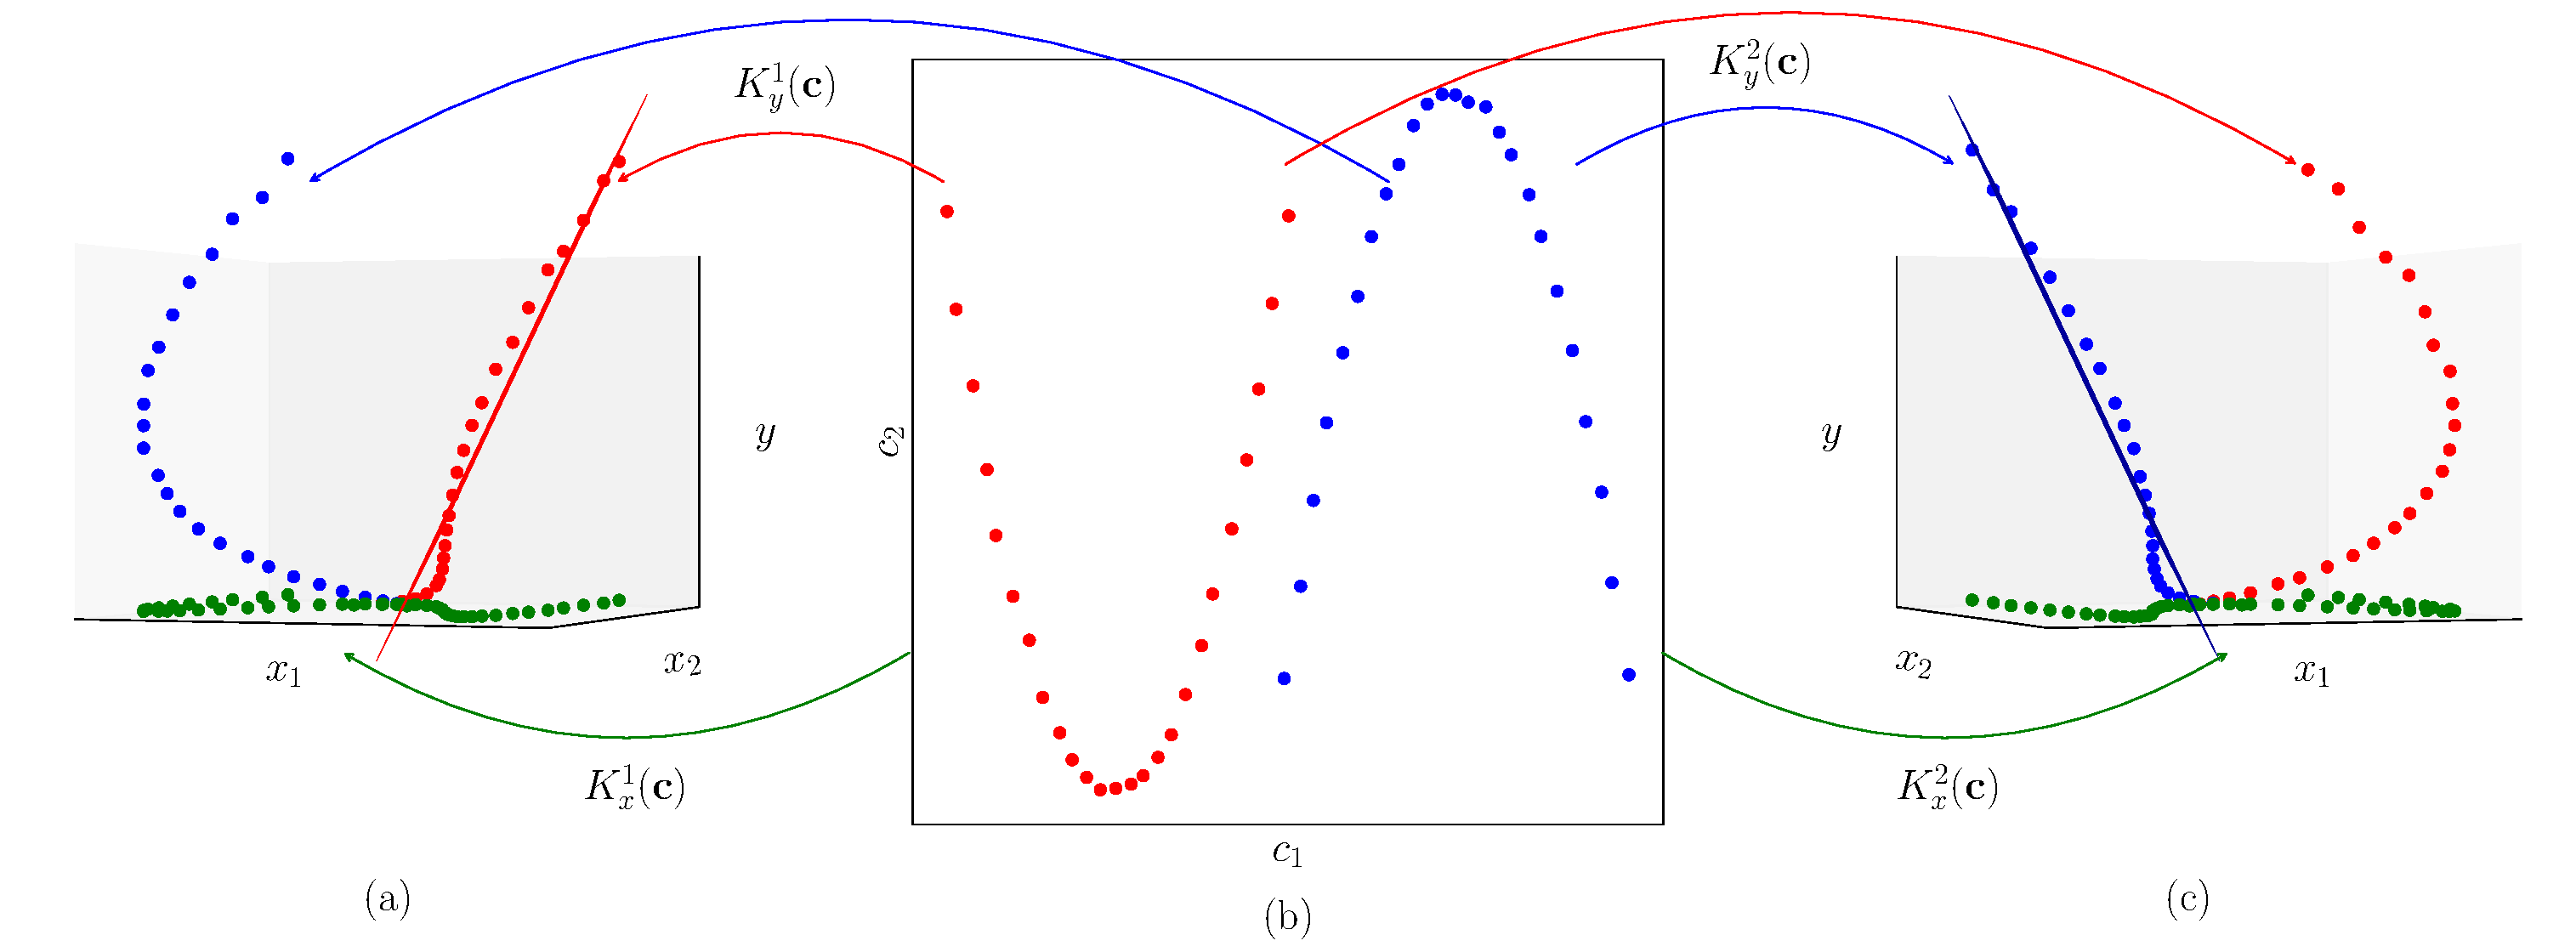
\includegraphics[width=\textwidth]{results/priorexpertfig/explanation}
     \caption{Пример: а) экспертная информация первого эксперта; б) исходные данные; в) экспертная информация второго эксперта}
    \label{intro:fig2}
\end{figure}
На рисунке \ref{intro:fig2} показан пример кривых второго порядка, а также экспертная информация о кривых. На рисунке \ref{intro:fig2}.a показана экспертная информация первого эксперта. Используя эту информацию, первая кривая аппроксимируется линейной моделью, а вторая кривая - шумом. На рисунке \ref{intro:fig2}.b показана экспертная информация второго эксперта. Используя эту информацию, вторая кривая аппроксимируется линейной моделью, а первая кривая представляет собой шум.

При аппроксимации нескольких кривых на одном контурном изображении строится многомодель. Примером нескольких моделей является случайный лес (Chen et al. 2012), бустинг деревьев (Chen et al. 2016), смесь экспертов (Yuksel et al. 2012). В данной работе смесь экспертов рассматривается как мультимодель. Смесь экспертов - это мультимодель, которая линейно взвешивает локальные модели, которые аппроксимируют часть выборки. Значения весовых коэффициентов зависят от объекта, для которого делается прогноз. Для решения проблемы смеси  экспертов используется вариационный EM-алгоритм (Dempster et al. 1997; Bishop 2010; Peng et al. 1996). Смесь экспертов имеет множество применений в ряде приложений. В работе  (Estabrooks et al. 2001) решается задача классификации текстов. В работах (Cheung et al. 1995; Weigend et al. 2000; Cao 2003; Mossavat et al. 2010; Sminchisescu C et al. 2007; Tuerk 2001; Yumlu et al. 2003), используется смесь экспертов для прогнозировать временные ряды для распознавания речи, повседневной деятельности человека и прогнозирования стоимости ценных бумаг. В работе (Ebrahimpour et al. 2009) смесь экспертов рассмотрена для решения задачи распознавания рукописных чисел на изображениях.

В качестве примера рассматривается задача аппроксимации изображения радужной оболочки глаза. На рисунке \ref{intro:fig1:real} показан пример изображения, которое необходимо аппроксимировать. Рассматриваем обработанное изображение, которое дано в виде схемы, пример такого изображения показан на рисунке \ref{intro:fig1:outer}. На рисунке \ref{intro:fig1:outer} показаны две модели окружностей, которые аппроксимируют радужную оболочку глаза. Окружности - простой пример кривой второго порядка.

\begin{figure}[h!]
\center
	\subfloat[]{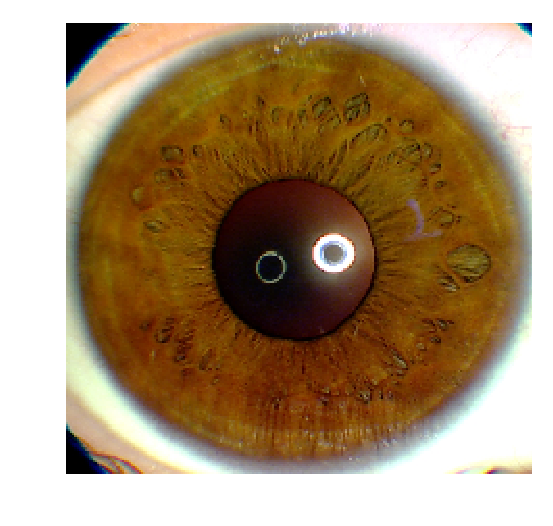
\includegraphics[height = 0.2\textheight]{results/priorexpertfig/real_image}\label{intro:fig1:real}} 
	\subfloat[]{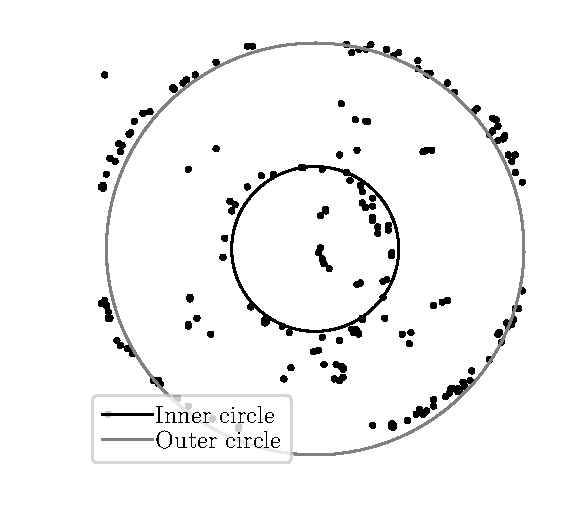
\includegraphics[height = 0.2\textheight]{results/priorexpertfig/outline_image}\label{intro:fig1:outer}} 
\caption{Пример изображения радужной оболочки глаза и ее контурное изображение: а) изображение радужной оболочки глаза; б) контурное изображение радужной оболочки и аппроксимация заданного изображения окружностей}
\label{intro:fig1}
\end{figure}

Для задачи аппроксимации радужной оболочки глаза используется следующая экспертная информация: радужная оболочка глаза аппроксимируется двумя концентрическими окружностями. Экспертная информация используется для построения описания характеристик точек на плоскости, а также для построения функции оптимизации. Часть функции ошибок для оптимизации, использующая экспертную информацию, называется регуляризатором. Таким образом, информация о том, что изображение окружностей задается описанием признака, и информация о том, что концентрические окружности задаются с помощью специального регуляризатора.

В вычислительном эксперименте качество аппроксимации контурного изображения анализируется в зависимости от заданной экспертной информации и от уровня шума в синтетически сгенерированных данных. Анализ качества аппроксимации диафрагмы проводится в зависимости от количества экспертной информации, которая использовалась при построении модели. Обратите внимание, что каждое приблизительное изображение представляет собой отдельный набор точек, которые необходимо приблизить.

\subsection{Постановка задачи поиска параметров кривых второго порядка}
Рассматривается бинарное изображение:
\[
\mathbf{M} \in \{0, 1 \}^{m_1\times m_2},
\]
где 1 соответствует черной точке изображения, а 0 соответствует белой точке фона.

Из изображения $\mathbf{M}$ строится выборка $\mathbf{C}$, элементами которой являются координаты $(x_i, y_i)$ черных точек:
\[
\mathbf{C} \in\mathbb{R}^{N \times 2}.
\]

Эксперт предполагает, что изображение состоит из кривой второго порядка $\Omega$.
Пусть для набора точек $\mathbf{C}\in\mathbb{R}^{N \times 2}$, образующих кривую $\Omega,$ дана экспертная информация о фигуре $E(\Omega)$ .
Множество $E(\Omega)$ состоит из формы $\Omega$, ожидаемой экспертом, и множества ее допустимых преобразований.

На основе экспертного описания введем отображения в новую задачу аппроксимации:
\[
\label{eq1}
	K_{x}\bigl(E(\Omega)\bigr): \mathbb{R}^{2} \rightarrow \mathbb{R}^{n}, \quad K_{y}\bigl(E(\Omega)\bigr): \mathbb{R}^{2} \rightarrow \mathbb{R},
\] 
где $K_{x}$ отображение объектов с признаковым описанием объектов, $n$ число признаков, а $K_{y}$ отображение в пространство целевых переменных для объекта. Применение отображений $K_{x}, K_{y}$ для всех элементов выборки $\mathbf{C}$:
\[
\label{eq2}
	K_{x}\bigl(E(\Omega\bigr), \mathbf{c}) = \mathbf{x}, \quad  K_{y}\bigl(E(\Omega), \mathbf{c}\bigr) = y,
\]
где $\mathbf{c} = (x_i, y_i)$ точки из выборки $\mathbf{C}$.

Применив отображения \eqref{eq2} к точкам $\mathbf{C}$ получаем выборку
\[
\label{eq4}
    \mathfrak{D} = \{(\mathbf{x}, y) \; | \; \forall \mathbf{c} \in \mathbf{C} \; \mathbf{x} = K_x(\mathbf{c}), \; y = K_y(\mathbf{c}) \}.
\]

Получаем, что исходная задача аппроксимации кривой $\Omega$ сводится к аппроксимации выборки $\mathfrak{D} $. В этой статье предполагается, что выборка $\mathfrak{D}$ аппроксимируется линейной моделью:
\[
	g(\mathbf{x}, \mathbf{w}) = \mathbf{x}^\mathsf{T} \mathbf{w},
\] 
где $\mathbf{w}$ вектор параметров, который необходимо найти.

Чтобы найти оптимальный вектор параметров $\hat{\mathbf{w}}$, необходимо решить следующую оптимизационную задачу:
\[
	\hat{\mathbf{w}} = \arg\min_{\mathbf{w}\in\mathbb{R}^n} \sum_{\left(\mathbf{x}, y\right) \in \mathfrak{D}}\|g(\mathbf{x}, \mathbf{w}) - y \|_2^2.
\] 

Таким образом, задача аппроксимации исходной кривой $\Omega$ сводится к решению задачи линейной регрессии, т.е. нахождению компонентов вектора $\hat{\mathbf{w}}$.

В случае, когда на изображении $K$ кривые второго порядка $\Omega_1, \dots, \Omega_K $, для каждой из которых есть экспертная информация $E_k = E(\Omega_k), \, k \in \{ 1, \dots, K \} $ ставится задача построения мультимодели, называемой смесью $ K $ экспертов.

\begin{definition}
Мультимодель $ f $ называется смесью K экспертов
\[
	f = \sum\limits_{k = 1}^{K}\pi_k(\mathbf{x}, \mathbf{V})g_k(\mathbf{w}_k),  \quad \pi_k(\mathbf{x}, \mathbf{V}): \mathbb{R}^{n\times |\mathbf{V}|} \rightarrow [0, \, 1], \quad \sum\limits_{k = 1}^{K}\pi_k(\mathbf{x}, \mathbf{V}) = 1, 
\]
где $g_k$ является локальной моделью~--- экспертом, а $\mathbf{x}$ является признаковым описанием объекта, $\pi_k$~--- шлюзовая функция, вектор $\mathbf{w}_k$ является параметрами локальной модели, а матрица $\mathbf{V}$ является параметрами шлюзовую функции.
\end{definition}

Для каждой кривой второго порядка даны отображения (\ref{eq1}). Для удобства введем следующие обозначения: $ K_x^k \bigr(\mathbf{c} \bigr) = K_x \bigr (\Omega_k, \mathbf{c} \bigr) $ и $K_y^k \bigr (\mathbf{c}\bigr) = K_y\bigr(\Omega_k, \mathbf{c}\bigr)$.
Затем с помощью локальных линейных моделей строится универсальная мультимодель, описывающая кривые $\Omega_1, \dots, \Omega_K$ на изображении $\mathbf{M}$:

\[
\label{5}
	f = \sum\limits_{\mathbf{c} \in \mathbf{C}} \sum_{k = 1}^{K} \pi_k(\mathbf{c}, \mathbf{V})g_k(K^k_{x}\bigl(\mathbf{c}), \mathbf{w}_k), 
\]
где $\pi_k$ задает шлюзовую функцию. Рассматривается случай, когда $\mathbf{x}=K^1_{x}\bigl(\mathbf{c})=\cdots=K^K_{x}\bigl(\mathbf{c}),$ то есть выражение \eqref{5} переписывается в следующей простой форме:
\[
\label{5_1}
	f = \sum\limits_{\mathbf{c} \in \mathbf{C}} \sum_{k = 1}^{K} \pi_k(\mathbf{x}, \mathbf{V})g_k(\mathbf{x}, \mathbf{w}_k), 
\]
где шлюзовая функция  $\pi_k$ имеет следующий вид:
\[
\label{6}
	\pi_k(\mathbf{x}, \mathbf{V}): \mathbb{R}^{n\times |\mathbf{V}|} \rightarrow [0, \, 1], \; \; \; \; \sum\limits_{k = 1}^{K}\pi_k(\mathbf{x}, \mathbf{V}) = 1,
\]
где $\mathbf{V}$ - параметры шлюзовой функции, а $ g_k $ - локальная модель.
    
Рассматривается следующий вид функций:
\[
    \boldsymbol{\pi}(\mathbf{x}, \mathbf{V}) = \text{softmax}\bigl(\mathbf{V}_1^{\mathsf{T}}\boldsymbol{\sigma}(\mathbf{V}_2^{\mathsf{T}}\mathbf{x}) \bigr),
\]
где $\mathbf{V} = \{ \mathbf{V}_1, \, \mathbf{V}_2\}$ параметры шлюзовой функцииs,
$\mathbf{V}_1 \in \mathbb{R}^{p \times k}, \, \mathbf{V}_2 \in \mathbb{R}^{n \times p}$. 

Чтобы найти оптимальные параметры мультимодели, необходимо решить следующую оптимизационную задачу:
\[\label{9}
\mathcal{L} = \sum\limits_{(\mathbf{x}, y) \in \mathfrak{D}} \sum\limits_{k = 1}^{K} \pi_k(\mathbf{x}, \mathbf{V})(y - \mathbf{w}_k^{\mathsf{T}}\mathbf{x})^2 + R\bigl(\mathbf{V}, \mathbf{W}, E(\Omega)\bigr) \rightarrow \min_{\mathbf{V}, \mathbf{W}},
\]
где $\mathbf{W} = [\mathbf{w}_1, \dots, \mathbf{w}_k]$~--- параметры локальных моделей, $R\bigl(\mathbf{V}, \mathbf{W}, E(\Omega)\bigr)$ регуляризационный параметр на основе экспертной информации.

\paragraph{Единое пространство для кривых второго порядка.} Произвольная кривая второго порядка, главная ось которой не параллельна оси ординат, задается следующим выражением:
\[
\label{st:coef}
x^2 = B'xy+C'y^2+D'x+E'y+F',
\]
где на коэффициенты $B', C'$ действуют ограничения, зависящие от типа кривой. Выражение \eqref{eq2} принимает следующий вид:
\[
\label{st:K_map}
K_x\bigr(\mathbf{c}_i\bigr)=\left[x_iy_i, y_i^2, x_i, y_i, 1\right], \quad K_y\bigr(\mathbf{c}_i\bigr)=x_i^2,
\]
откуда получается задача линейной регрессии для восстановления параметров $B', C', D', E', F'$ по выбранной выборке.

\paragraph{Окружность.} Как частный случай кривой второго порядка, рассматривается окружность.
Пусть $(x_0, y_0)$ - это центр окружности, которую нужно найти на бинарном изображении $\mathbf{M}$, а $r$ - его радиус.
Элементы $(x_i, y_i)\in\mathbf{C}$ представляют собой геометрическое место точек, которое аппроксимируется уравнением окружности:
\[
(x_i - x_0)^2 + (y_i - y_0)^2 = r^2.
\]
Раскладывая скобки, получаем:
\[(2x_0)\cdot x_i + (2y_0)\cdot y_i + (r^2 - x_0^2 - y_0^2)\cdot 1 = x_i^2 + y_i^2 . 
\]
Тогда выражение \eqref{eq2} принимает следующий вид:
\[
\label{10}
K_{x}(\mathbf{c}_i) = [x_i, \, y_i, \, 1] = \mathbf{x}, \,  K_{y}(\mathbf{c}_i) = x_i^2+y_i^2 = y.
\] 
Получаем задачу линейной регрессии \eqref{eq4}.
Компоненты вектора $\mathbf{w} = [w_0, \, w_1, \, w_2]^\mathsf{T}$ связывают признаковое описание $\mathbf{x}$ и целевую переменную $y$. Параметры окружности, через параметры линейной модели: \[ x_0 = \frac{w_0}{2}, \; y_0 = \frac{w_1}{2}, \; r = \sqrt{w_3 + x_0^2 + y_0 ^2}.\]

\subsection{Композиция кривых второго порядка на изображении}
\label{sec:4}
Для построения композиции из фигур воспользуемся выражением \eqref{9}, которое принимает следующий вид:
\[ 
\label{statment:optim:task}
\begin{aligned}
\mathcal{L} = \sum\limits_{\mathbf{c} \in \mathbf{C}} \sum\limits_{k = 1}^{K} \pi_k(\mathbf{c}, \mathbf{V})\left(K^{k}_y\bigr(\mathbf{c}\bigr) - \mathbf{w}_k^{\mathsf{T}}K^{k}_x\bigr(\mathbf{c}\bigr)\right)^2 + R\bigl(\mathbf{V}, \mathbf{W}, E(\Omega)\bigr) \rightarrow \min_{\mathbf{V}, \mathbf{W}},
\end{aligned}
\] 
где $K^{k}_x, K^{k}_y$ экспертное представление $k$-го эксперта. Предполагая, что все кривые на изображении описываются одним признаковым описанием $\mathbf{x} =K^{1}_x\bigr(\mathbf{c}\bigr)=\cdots=K^{K}_x\bigr(\mathbf{c}\bigr), x= K^{1}_y\bigr(\mathbf{c}\bigr)=\cdots=K^{K}_y\bigr(\mathbf{c}\bigr),$ получаем следующую задачу оптимизации:
\[ 
\label{statment:optim:task:simp}
\begin{aligned}
\mathcal{L} = \sum\limits_{\left(\mathbf{x}, y\right) \in \mathfrak{D}} \sum\limits_{k = 1}^{K} \pi_k(\mathbf{x}, \mathbf{V})\left(y - \mathbf{w}_k^{\mathsf{T}}\mathbf{x}\right)^2 + R\bigl(\mathbf{V}, \mathbf{W}, E(\Omega)\bigr) \rightarrow \min_{\mathbf{V}, \mathbf{W}},
\end{aligned}
\] 

В качестве регуляризатора $R$ рассматриваются дополнительные ограничения на векторы параметров модели. Для решения задачи оптимизации \eqref{statment:optim:task:simp} предлагается использовать EM-алгоритм.

\subsection{Анализ смеси экспертов для аппроксимации кривых второго порядка на изображении}
\label{sec:5}

Проведен вычислительный эксперимент по анализу качества моделей кривых второго порядка на изображении. Эксперимент разделен на несколько частей. Первая часть - это эксперимент с несколькими окружностями на изображении. Во второй части анализируется сходимость метода в зависимости от уровня шума в данных и от указанной экспертной информации. В третьей части проводится эксперимент по аппроксимации радужной оболочки глаза.

\begin{figure}[h!]
\center
	\subfloat[]{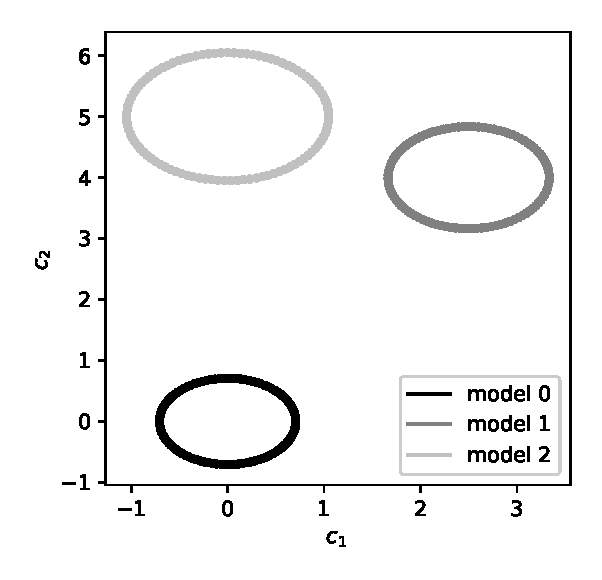
\includegraphics[height = 0.2\textheight]{results/priorexpertfig/900.eps}} 
	\subfloat[]{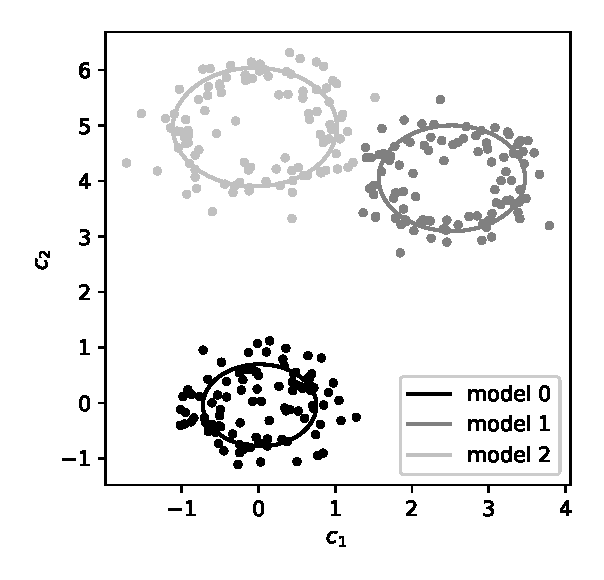
\includegraphics[height = 0.2\textheight]{results/priorexpertfig/901.eps}}
	\subfloat[]{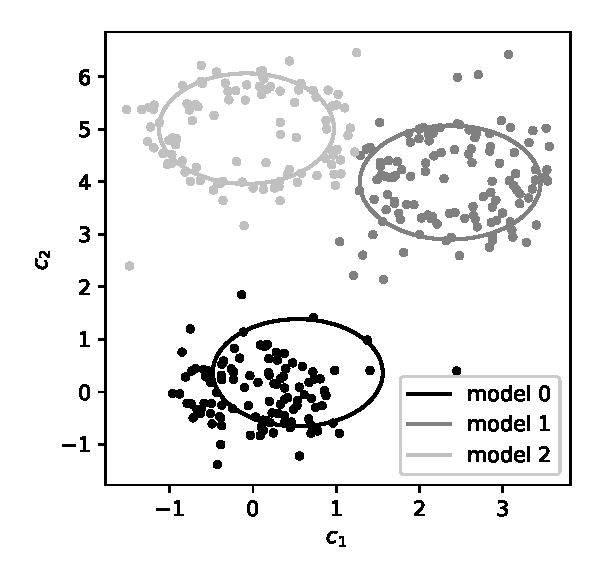
\includegraphics[height = 0.2\textheight]{results/priorexpertfig/902.eps}} 
\caption{Мультимодель в зависимости от различных предварительных предположений и уровня шума. Слева направо: окружности без шума; шум в радиусе круга; шум в радиусе круга, а также произвольные точки по всему изображению.}
\label{ce:fig3}
\end{figure}

\begin{figure}[h]
\center
	\subfloat[]{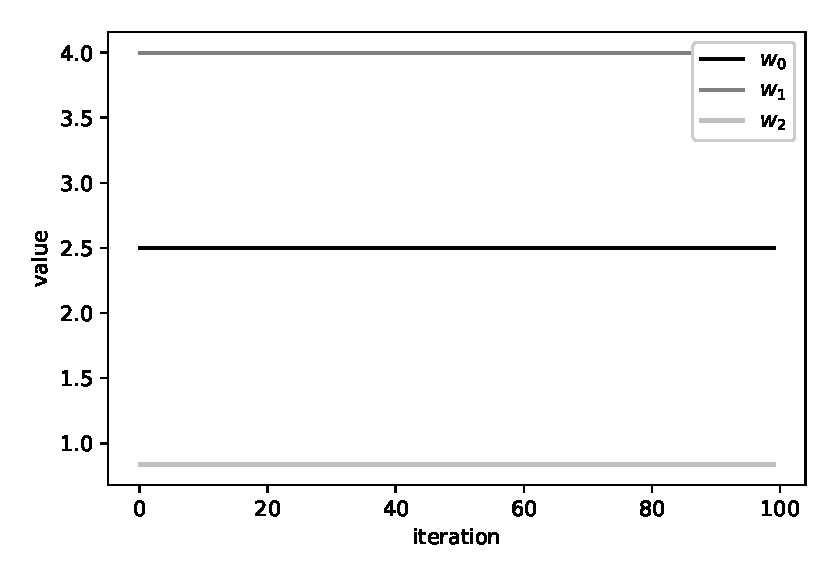
\includegraphics[height = 0.2\textheight]{results/priorexpertfig/900noise.eps}} 
	\subfloat[]{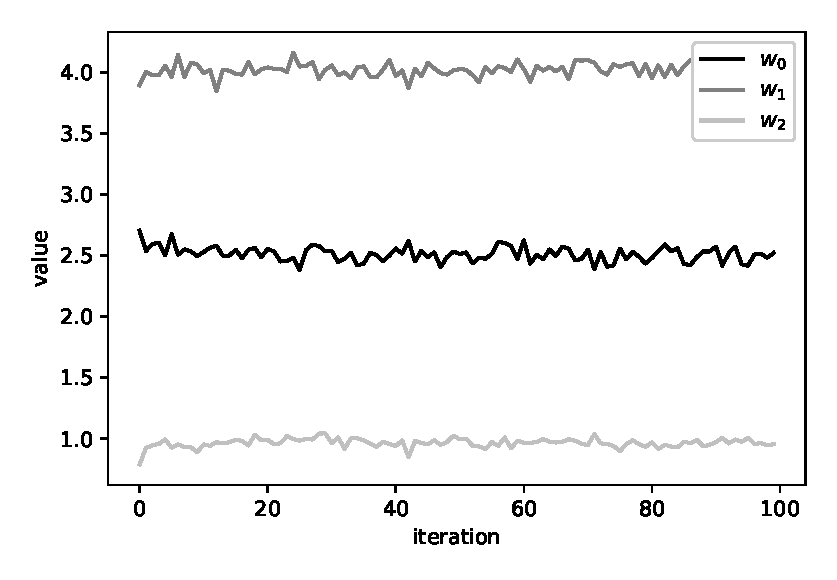
\includegraphics[height = 0.2\textheight]{results/priorexpertfig/901noise.eps}}\\
	\subfloat[]{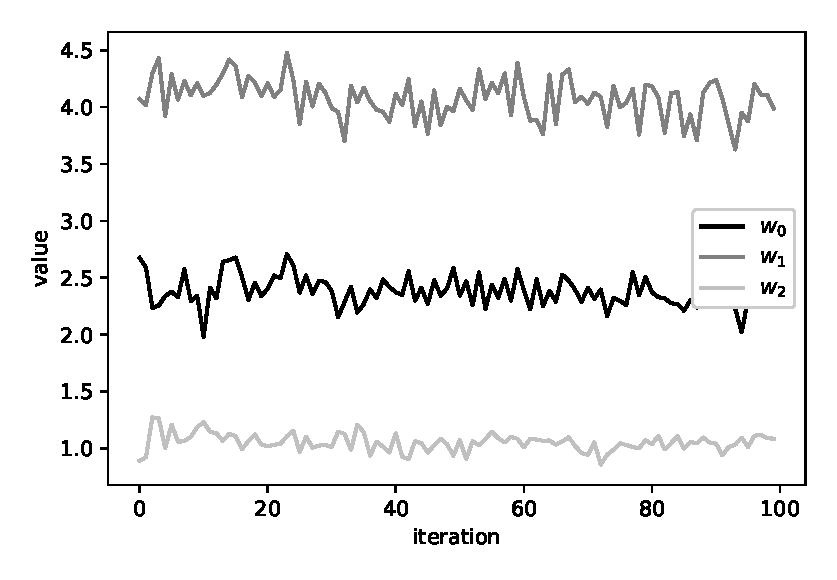
\includegraphics[height = 0.2\textheight]{results/priorexpertfig/902noise.eps}} 

\caption{Зависимость параметров $r$, $x_0$ и $y_0$ от номера итерации для различных априорных распределений. Слева направо: окружности без шума; шум в радиусе круга; шум в радиусе круга, а также произвольные точки по всему изображению.}
\label{ce:fig4}
\end{figure}

В этой части эксперимента показан пример обучения мультимодели для аппроксимации нескольких фигур второго порядка одновременно. В качестве данных используется синтетическая выборка, который получается путем создания трех произвольных непересекающихся окружностей, а также добавления шума к этим окружностям. Шум был добавлен к радиусу круга для каждой точки, а также случайные точки были добавлены к выборке.

На рисунке \ref{ce:fig3} показан результат построения ансамбля локально аппроксимирующих моделей, которые аппроксимируют образец. Каждая локальная модель аппроксимирует одну окружность, а при добавлении еще большего шума качество аппроксимации падает.
На рисунке \ref{ce:fig4} показан график зависимости радиуса окружностей $ r $ и их центров $(x_0, y_0)$ от номера итерации.

\begin{figure}[h!t]
\center
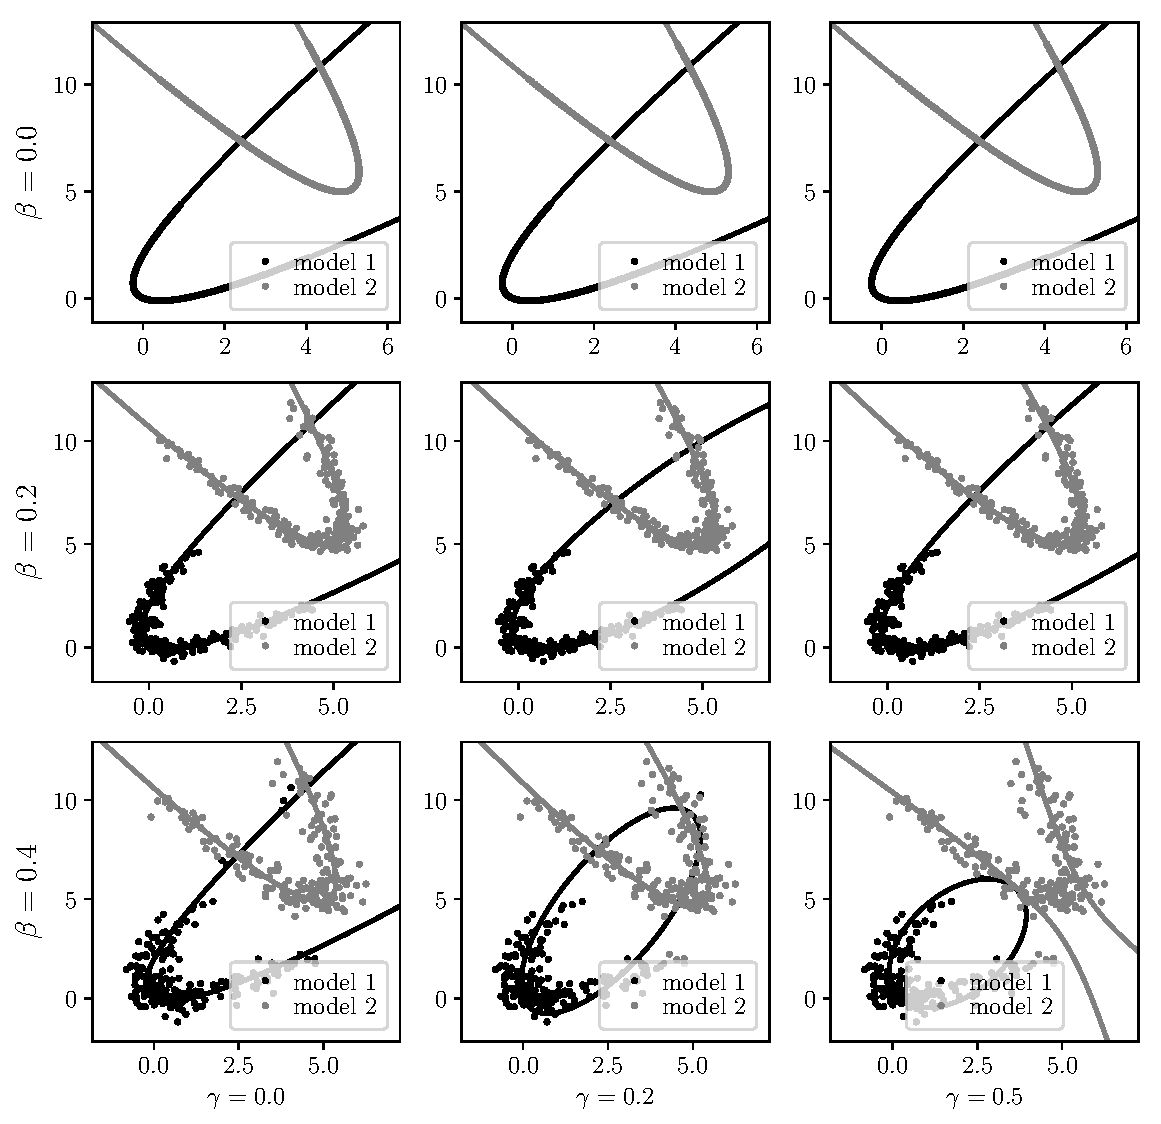
\includegraphics[width=0.8\textwidth]{results/priorexpertfig/beta_gamma}
\caption{Результат аппроксимации для данных с разными уровнями шума $\beta$ и дисперсией априорного распределения $\gamma$}
\label{ce:fig6}
\end{figure}

\begin{figure}[h!t]
\center
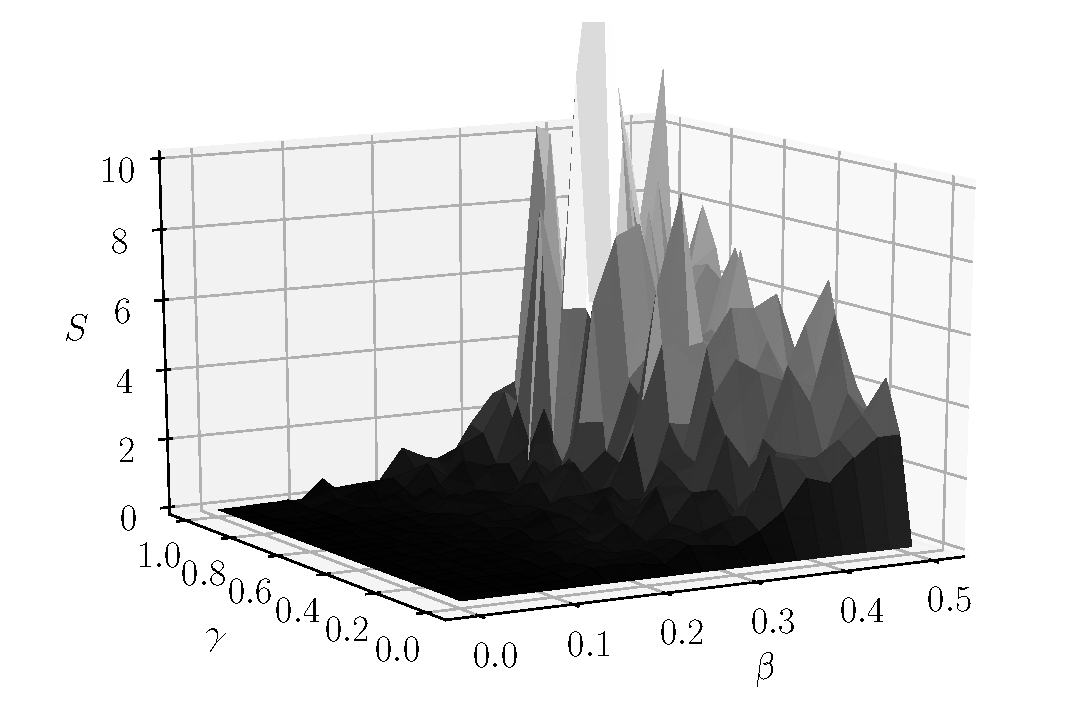
\includegraphics[width=0.5\textwidth]{results/priorexpertfig/3dplot}
\caption{Зависимость моделей от уровня шума $\beta$ в данных, а также от дисперсии априорного распределения $\gamma$}
\label{ce:fig5}
\end{figure}

В этой части эксперимента анализируется качество аппроксимации $S$ в зависимости от уровня шума $\beta$ в данных и по параметру априорных распределений $\gamma$. Пример получается следующим образом: сначала случайным образом выбираются два вектора параметров: $\mathbf{w}^\text{true}_{1}$ и $\mathbf{w}^\text{true}_{2}$ коэффициенты двух парабол. Векторы $\mathbf{w}^\text{true}_{1}$ и $\mathbf{w}^\text{true}_{2}$ используются для создания точек $x_i$ и $y_i$ с добавлением нормального шума $\varepsilon\sim\mathcal{N}\bigr(0, \beta\bigr) $. При обучении мультимодели, априорное распределение параметров считается $\mathbf{w}_1\sim\mathcal{N}\bigr(\mathbf{w}^\text{true}_{1}, \gamma\mathbf{I}\bigr), \mathbf{w}_2\sim\mathcal{N}\bigr(\mathbf{w}^\text{true}_{2},\gamma\mathbf{I}\bigr)$.

Рассмотри критерий качества:
\[
S = ||\mathbf{w}^\text{pred}_{1} - \mathbf{w}^\text{true}_{1}||^{2}_{2} + ||\mathbf{w}^\text{pred}_{2} - \mathbf{w}^\text{true}_{2}||^{2}_{2},
\]
где $\mathbf{w}^\text{pred}_{1}$ аппроксимация вектора параметров первой локальной модели, а $\mathbf{w}^\text{pred}_{2} $ аппроксимация вектора параметров второй локальной модели.

На рисунке \ref{ce:fig5} показана зависимость критерия качества $S$ от уровня шума $\beta$ и параметра априорного распределения $\gamma$. График показывает, что при низком уровне шума $\beta$ качество приближения не зависит от параметра $\gamma$, а с увеличением шума $\beta$ качество приближения $S$ снижается.

На рисунке \ref{ce:fig5} показан пример того, как алгоритм работает с разными параметрами $\beta$ и $\gamma$. Видно, что в отсутствие шума $\beta$ обе локальные модели аппроксимируют образец. С увеличением уровня шума качество аппроксимации снижается: при $\beta = 0{,}2$ при увеличении $\gamma$ первая локальная модель от параболы переходит в эллипс; при $\beta = 0{,}4$ при увеличении $\gamma$ первая локальная модель из параболы переходит в эллипс, а вторая модель из параболы переходит в гиперболу.

\begin{figure}[h!]
\center
	\subfloat[]{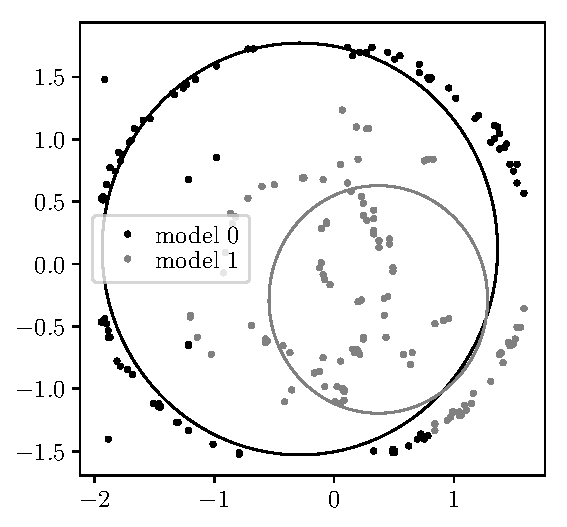
\includegraphics[height = 0.17\textheight]{results/priorexpertfig/not_prior_real_example}} 
	\subfloat[]{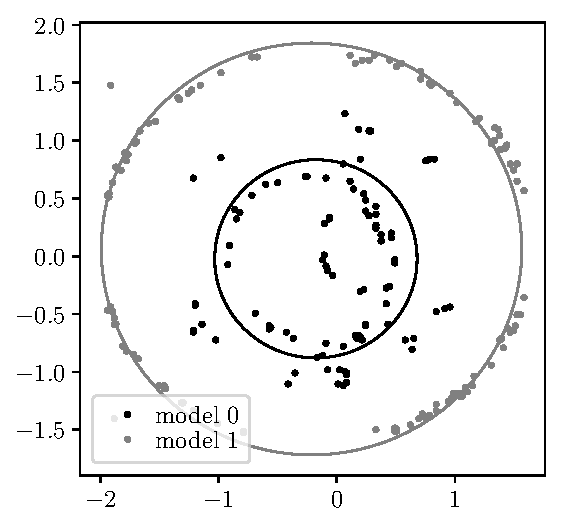
\includegraphics[height = 0.17\textheight]{results/priorexpertfig/prior_real_example}}
	\subfloat[]{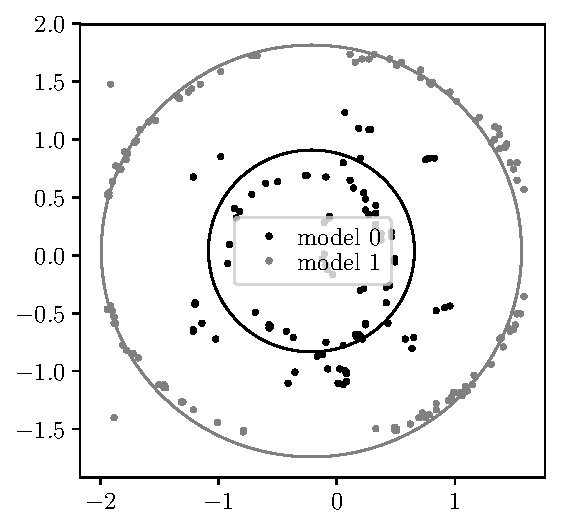
\includegraphics[height = 0.17\textheight]{results/priorexpertfig/prior_regular_real_example}} 
\caption{Визуализация приближения радужной оболочки: а) если указан регуляризатор $ R_0 $; б) если указан регуляризатор $ R_1 $; б) если указан регуляризатор $ R_2 $}
\label{ce:fig6}
\end{figure}


\begin{figure}
\center
     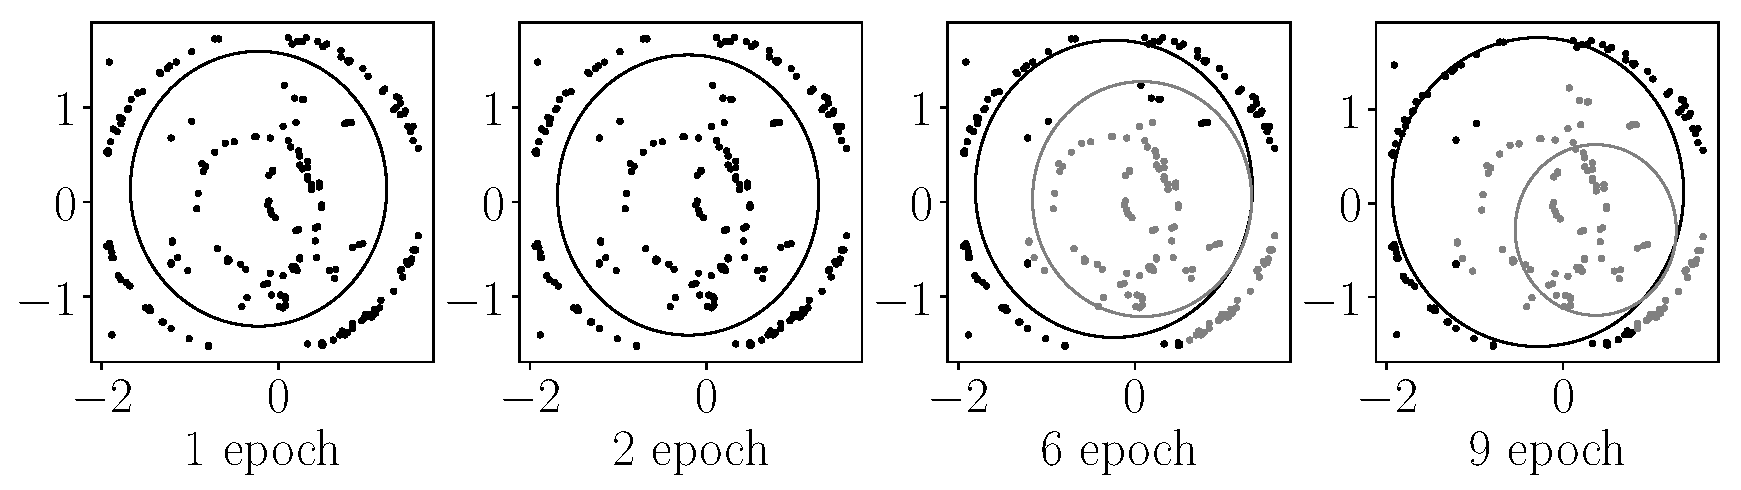
\includegraphics[width=\textwidth]{results/priorexpertfig/experiment_real_not_prior}\\
     \caption{Визуализация процесса сходимости параметров мультимодели в случае регуляризатора $ R_0 $}
    \label{ce:fig7}
\end{figure}

\begin{figure}
\center
     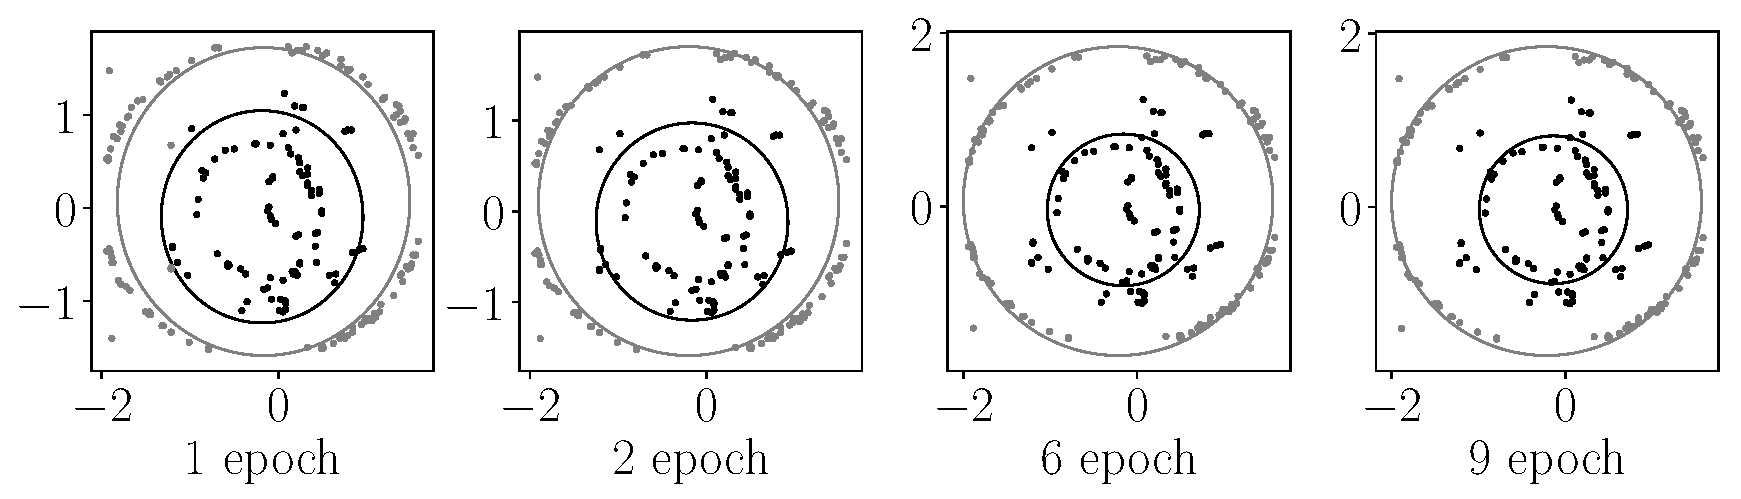
\includegraphics[width=\textwidth]{results/priorexpertfig/experiment_real_prior}
     \caption{Визуализация процесса сходимости параметров мультимодели в случае регуляризатора $ R_1 $}
    \label{ce:fig8}
\end{figure}

\begin{figure}
\center
     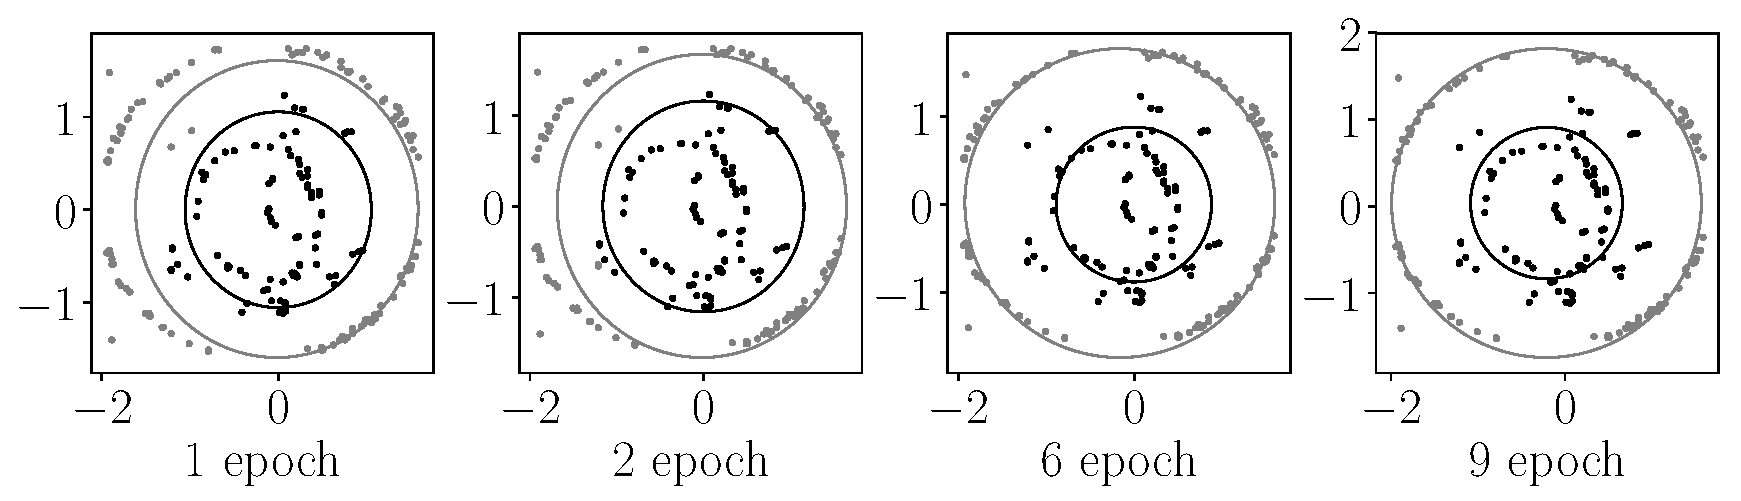
\includegraphics[width=\textwidth]{results/priorexpertfig/experiment_real_regular}
     \caption{Визуализация процесса сходимости параметров мультимодели в случае регуляризатора $ R_2 $}
    \label{ce:fig9}
\end{figure}

Анализ качества аппроксимации проводится для задачи аппроксимации радужной оболочки глаза на изображении. Радужная оболочка глаза состоит из двух концентрических окружностей, поэтому рассматривается мультимодель, состоящая из двух экспертов: каждый эксперт аппроксимирует одно из обстоятельств. В вычислительном эксперименте сравнивается качество аппроксимации окружностей при задании разных регуляризаторов $ R_0, R_1, R_2 $. Регуляризатор $ R_0 \bigl(\mathbf{V}, \mathbf{W}, E(\Omega) \bigr) = 0, $ то есть регуляризатора нет. Регуляризатор:

\[
R_1\bigl(\mathbf{V}, \mathbf{W}, E(\Omega)\bigr)= -\sum_{k=1}^{K}\mathbf{w}_k^{\mathsf{T}}\mathbf{w}_k,
\]
который удаляет околонулевые параметры локальных моделей.
Регуляризатор
\[
R_2\bigl(\mathbf{V}, \mathbf{W}, E(\Omega)\bigr)= -\sum_{k=1}^{K}\mathbf{w}_k^{\mathsf{T}}\mathbf{w}_k + \sum_{k=1}^{K}\sum_{k'=1}^{K}\sum_{j=1}^2\left(w_k^j-w_k'^j\right)^2,
\]
что способствует совпадению центров окружностей и близким к нулю параметрам модели.
На рисунке \ref{ce:fig6} показан результат алгоритма аппроксимации радужной оболочки глаза после 10 итераций. Видно, что при отсутствии регуляризатора одна из окружностей находится некорректно. Если задан регуляризатор $ R_1 $, модель аппроксимирует обе окружности с хорошим качеством, но окружности не концентрические. В случае задания регуляризатора $ R_2 $ мы получим концентрические окружности на изображении.

На рисунках \ref{ce:fig7}-\ref{ce:fig9} показан процесс сходимости мультимоделей в случае задания разных регуляризаторов $ R_0, R_1, R_2 $. Видно, что модели с типом регуляризатора $ R_1 $ и $ R_2 $ аппроксимируют обе окружности, а мультимодель с регуляризатором $ R_0 $ аппроксимирует только большую окружность.
